\chapter{Implementation}

\section{Policy}
The policy is composed of the following parts:

\begin{itemize}
	\item Hardware
	\item Kernel
	\item Binaries
	\item Subjects
	\item Scheduling
\end{itemize}

Each of the main policy parts is presented in the following sections. Preceding
these descriptions is the specification of data types, which are the basis for
the subsequent definition of policy elements.

\subsection{Data types}
This section describes basic data types that are used in the specification of
the system policy. They are referenced in later chapters, illustrating different
parts of the policy.

\input{types.tex}

\subsection{Hardware}
\begin{figure}[h]
	\centering
	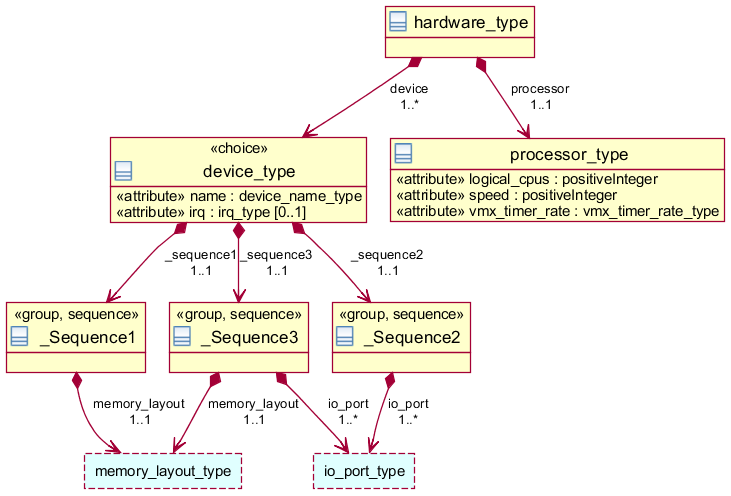
\includegraphics[width=\textwidth]{images/xml_hardware.png}
	\caption{Hardware policy}
\end{figure}
\input{hardware.tex}

\subsection{Kernel}
\begin{figure}[h]
	\centering
	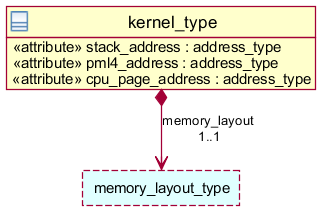
\includegraphics[scale=0.6]{images/xml_kernel.png}
	\caption{Kernel policy}
\end{figure}
\input{kernel.tex}

\subsection{Binaries}
\begin{figure}[h]
	\centering
	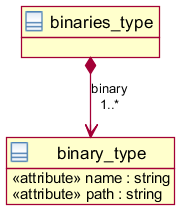
\includegraphics[scale=0.6]{images/xml_binary.png}
	\caption{Binaries policy}
\end{figure}
\input{binary.tex}

\subsection{Subjects}
\begin{sidewaysfigure}[hp]
	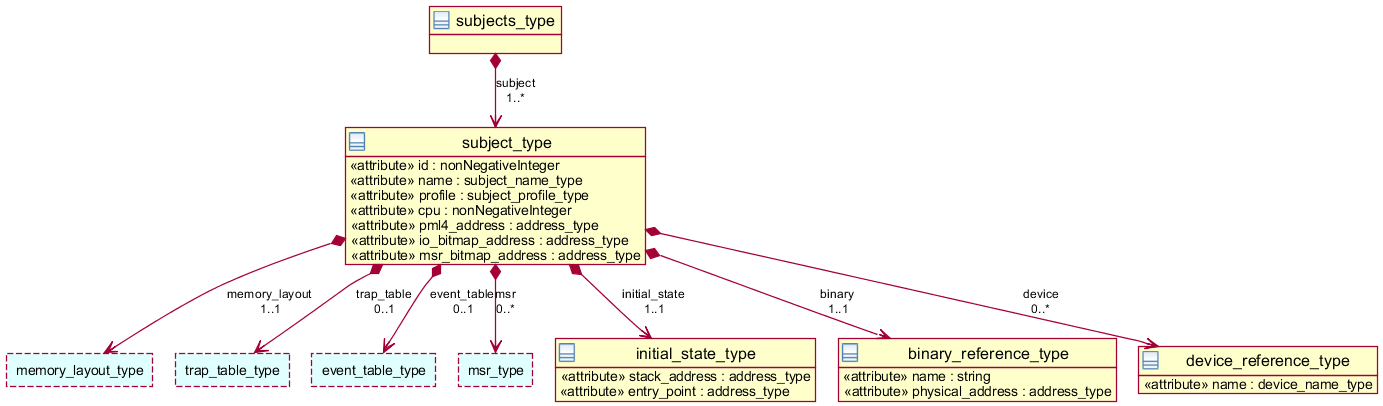
\includegraphics[width=\textwidth]{images/xml_subject.png}
	\caption{Subjects policy}
\end{sidewaysfigure}
\input{subject.tex}

\subsection{Scheduling}
\begin{figure}[h]
	\centering
	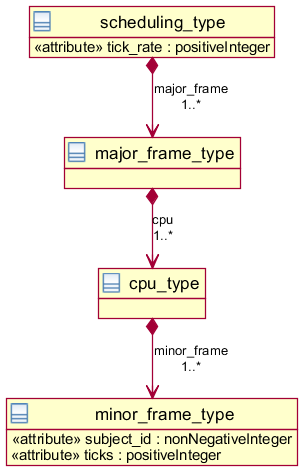
\includegraphics[scale=0.6]{images/xml_scheduling.png}
	\caption{Scheduling policy}
\end{figure}
\input{scheduling.tex}

\section{Kernel}
\subsection{Scheduling}
\subsection{Traps}
\subsection{Exceptions and Interrupts}
\subsection{Events}
\subsection{Multicore support}
\section{Build}
